\documentclass[norsk,a4paper,12pt]{article}
\usepackage[utf8]{inputenc}
\usepackage{graphicx} %for å inkludere grafikk
\usepackage{verbatim} %for å inkludere filer med tegn LaTeX ikke liker
\usepackage{tabularx}
\usepackage{booktabs}
\usepackage{amsmath}
\usepackage{float}
\usepackage{listings}
\usepackage{hyperref}
%\usepackage{subfigure}
\usepackage{subcaption}
\usepackage{caption}
\usepackage{color}
\usepackage[sep=3pt, offset=0.8em]{simpler-wick}
\usepackage{tikz}

\lstset{language=python}
\lstset{basicstyle=\small}
\lstset{backgroundcolor=\color{white}}
\lstset{frame=single}
\lstset{stringstyle=\ttfamily}
\lstset{keywordstyle=\color{red}\bfseries}
\lstset{commentstyle=\itshape\color{blue}}
\lstset{showspaces=false}
\lstset{showstringspaces=false}
\lstset{showtabs=false}
\lstset{breaklines}
\lstset{postbreak=\raisebox{0ex}[0ex][0ex]{\ensuremath{\color{red}\hookrightarrow\space}}}
%\usepackage{titlesec}

\setcounter{secnumdepth}{4}

%\titleformat{\paragraph}
%{\normalfont\normalsize\bfseries}{\theparagraph}{1em}{}
%\titlespacing*{\paragraph}
%{0pt}{3.25ex plus 1ex minus .2ex}{1.5ex plus .2ex}


\title{FYS-KJM4480 - Quantum mechanics for many-particle systems \\\vspace{2mm} \Large{Project 2}}
\author{\large Even Marius Nordhagen}
\date\today
\begin{document}

\maketitle

\begin{itemize}
\item For the Github repository containing programs and results, follow this link: 
\url{https://github.com/evenmn/master/tree/master/FYSKJM4480/Project2}
\end{itemize}

\section{Introduction}
Superconductivity might be one of 20th century's most exciting physical discoveries, and for a long time the theory behind was a mystery. In 1957, 46 years after the first observation by Kamerlingh Onnes, John Bardeen, Leon Cooper and John Robert Schrieffer came up with a quantum theory describing superconductivity on microscopic level. This theory was built on Cooper pairs, which is a pair of electrons with lower energy than the Fermi energy, i.e. there is a bounding between them. We can treat the pairs as a particle, which is a boson due to the total spin 1, and this boson-like pair is the reason why the current can flow unhindered in a superconductor. 

Furthermore the theory is also used in nuclear physics to describe the paring interaction between nucleons in an atomic nucleus. 

This project aims to study such a pairing model, known as BCS-theory after its founders. In the first part we are working with this model independently. Then we will use Configuration-Interaction Doubled (CID) as an approximation to make the equations computer-friendly, and thereafter we repeat this using Coupled-Cluster Doubled (CCD). Finally the results are compared for both the methods, and we will discuss why one method is better than the other.
\newpage

\section{Pairing model}
In this project we use a slightly simplified pairing model, which we assume to be carrying a constant strength $g$. The Hamiltonian is therefore given by
\begin{equation}
\hat{H}=\hat{H}_0+\hat{V}
\end{equation}
with
\begin{equation}
\hat{H}_0=\sum_{p\sigma}\epsilon_pc_{p\sigma}^{\dagger}c_{p\sigma},\quad \epsilon_p=\xi\cdot(p-1)
\end{equation}
and
\begin{equation}
\hat{V}=-\frac{1}{2}g\sum_{pq}c_{p+}^{\dagger}c_{p-}^{\dagger}c_{q-}c_{q+}.
\end{equation}

We will only study systems of a even number of particles, $N$, and the ground-state wavefunction is then given by the Slater determinant
\begin{equation}
|\Phi\rangle=c_{1+}^{\dagger}c_{1-}^{\dagger}\hdots c_{N/2 +}^{\dagger}c_{N/2 -}^{\dagger}|\Phi\rangle.
\end{equation}
Further I will define some operators that will be useful when doing the calculations. 
\begin{equation}
\hat{P}_p^{\dagger}\equiv c_{p+}^{\dagger}c_{p-}^{\dagger},\quad \hat{P}_p\equiv c_{p-}c_{p+}
\end{equation}
\begin{equation}
\hat{n}_p\equiv\sum_{\sigma}c_{p\sigma}^{\dagger}c_{p\sigma}
\end{equation}
\begin{equation}
\hat{P}=\sum_p\hat{P}_p^{\dagger}\hat{P}_p
\end{equation}
and finally
\begin{equation}
\hat{S}_z=\frac{1}{2}\sum_{p\sigma}\sigma c_{p\sigma}^{\dagger}c_{p\sigma}.
\end{equation}

\subsection{Exercise 1A}
\subsection{Exercise 1B}
\subsection{Exercise 1C}
\subsection{Exercise 1D}
\begin{equation}
[\hat{P}_p,\hat{P}_q^{\dagger}]=\hat{P}_p\hat{P}_q^{\dagger}-\hat{P}_q^{\dagger}\hat{P}_p
\end{equation}
Will only include terms which contribute, and we obtain
\begin{align}
\hat{P}_p\hat{P}_q^{\dagger}&=\sum_{pq}c_{p-}c_{p+}c_{q+}^{\dagger}c_{q-}^{\dagger}\notag\\
&=\{c_{q+}^{\dagger}c_{q-}^{\dagger}c_{p-}c_{p+}\}+\{\wick{\c c_{p-}c_{p+}c_{q+}^{\dagger}\c c_{q-}^{\dagger}}\}+\{\wick{c_{p-}\c c_{p+}\c c_{q+}^{\dagger}c_{q-}^{\dagger}}\}+\{\wick{\c2 c_{p-}\c1 c_{p+}\c1 c_{q+}^{\dagger}\c2 c_{q-}^{\dagger}}\}\notag\\
&=\{c_{q+}^{\dagger}c_{q-}^{\dagger}c_{p-}c_{p+}\}-\delta_{pq}c_{p+}c_{q+}^{\dagger}-\delta_{pq}c_{p-}c_{q-}^{\dagger}+\delta_{pq}\delta_{pq}
\end{align}
due to Wick's theorem. Several terms vanish since a delta function of operators of opposite spin does not contribute, i.e. $\delta_{p+q-}=0$. Calculating $\hat{P}_q^{\dagger}\hat{P}_p$ is a simple task:
\begin{equation}
\hat{P}_q^{\dagger}\hat{P}_p=\{c_{q+}^{\dagger}c_{q-}^{\dagger}c_{p-}c_{p+}\}.
\end{equation}
Furthermore we will omit the spin in delta functions, because it does not affect the delta function as long as the spin is equally directed. We set $p=q$, but not in the Dirac delta functions:
\begin{align}
\hat{P}_p\hat{P}_q^{\dagger}-\hat{P}_q^{\dagger}\hat{P}_p&=-\delta_{pq}c_{q+}^{\dagger}c_{q+}-\delta_{pq}c_{q-}^{\dagger}c_{q-}+\delta_{pq}\delta_{qq}\notag\\
&=\delta_{pq}(1-c_{q+}^{\dagger}c_{q+}-c_{q-}^{\dagger}c_{q-})\notag\\
&=\delta_{pq}(1-\hat{n}_q)
\end{align}

\subsection{e}
We have $N=4$, thus 
\begin{align}
|\Phi\rangle&=c_{1+}^{\dagger}c_{1-}^{\dagger}c_{2+}^{\dagger}c_{2-}^{\dagger}|-\rangle\\
&=\hat{P}_1^{\dagger}\hat{P}_2^{\dagger}|-\rangle.
\end{align}
$M$ is the number of states, with $p$ as an index
\begin{align}
\hat{P}&=\sum_{p=1}^M\hat{P}_p^{\dagger}\hat{P}_p\\
&=\hat{P}_1^{\dagger}\hat{P}_1+\hat{P}_2^{\dagger}\hat{P}_2+\hat{P}_3^{\dagger}\hat{P}_3+\hat{P}_4^{\dagger}\hat{P}_4
\end{align}
since $M=4$. 
\begin{align}
\hat{P}|\Phi\rangle&=\Big(\hat{P}_1^{\dagger}\hat{P}_1\hat{P}_1^{\dagger}\hat{P}_2^{\dagger}+\hat{P}_2^{\dagger}\hat{P}_2\hat{P}_1^{\dagger}\hat{P}_2^{\dagger}+...\Big)|-\rangle\\
&=\Big(\delta_{11}\hat{P}_1^{\dagger}\hat{P}_2^{\dagger}+\delta_{22}\hat{P}_1^{\dagger}\hat{P}_2^{\dagger}\Big)|-\rangle\\
&=2|\Phi\rangle
\end{align}
where the two last terms in $\hat{P}$ do not contribute since $|\Phi\rangle$ does not contain creation operators with index 3 or 4. This computation was quite short since we could replace all operators with $\hat{P}$ which is not always the case, something we will see when calculating $\hat{S}_z|\Phi\rangle$.
\begin{align}
\hat{S}_z=&\frac{1}{2}\sum_{p\sigma}\sigma c_{p\sigma}^{\dagger}c_{p\sigma}\\
=&\frac{1}{2}\Big(c_{1+}^{\dagger}c_{1+}-c_{1-}^{\dagger}c_{1-}+c_{2+}^{\dagger}c_{2+}-c_{2-}^{\dagger}c_{2-}+\notag\\
&c_{3+}^{\dagger}c_{3+}-c_{3-}^{\dagger}c_{3-}+c_{4+}^{\dagger}c_{4+}-c_{4-}^{\dagger}c_{4-}\Big)|-\rangle
\end{align}
\begin{align}
\hat{S}_z|\Phi\rangle=&\frac{1}{2}\Big(c_{1+}^{\dagger}c_{1+}c_{1+}^{\dagger}c_{1-}^{\dagger}c_{2+}^{\dagger}c_{2-}^{\dagger}-c_{1-}^{\dagger}c_{1-}c_{1+}^{\dagger}c_{1-}^{\dagger}c_{2+}^{\dagger}c_{2-}^{\dagger}\notag\\
&+c_{2+}^{\dagger}c_{2+}c_{1+}^{\dagger}c_{1-}^{\dagger}c_{2+}^{\dagger}c_{2-}^{\dagger}-c_{2-}^{\dagger}c_{2-}c_{1+}^{\dagger}c_{1-}^{\dagger}c_{2+}^{\dagger}c_{2-}^{\dagger}\Big)|-\rangle\\
=&\frac{1}{2}\Big(\wick{c_{1+}^{\dagger}\c1 c_{1+}\c1 c_{1+}^{\dagger}c_{1-}^{\dagger}c_{2+}^{\dagger}c_{2-}^{\dagger}-c_{1-}^{\dagger}\c2 c_{1-}c_{1+}^{\dagger}\c2 c_{1-}^{\dagger}c_{2+}^{\dagger}c_{2-}^{\dagger}}\notag\\
&\wick{+c_{2+}^{\dagger}\c3 c_{2+}c_{1+}^{\dagger}c_{1-}^{\dagger}\c3 c_{2+}^{\dagger}c_{2-}^{\dagger}-c_{2-}^{\dagger}\c4 c_{2-}c_{1+}^{\dagger}c_{1-}^{\dagger}c_{2+}^{\dagger}\c4 c_{2-}^{\dagger}}\Big)|-\rangle\\
=&\frac{1}{2}\Big(\delta_{1+1+}c_{1+}^{\dagger}c_{1-}^{\dagger}c_{2+}^{\dagger}c_{2-}^{\dagger}-\delta_{1-1-}c_{1+}^{\dagger}c_{1-}^{\dagger}c_{2+}^{\dagger}c_{2-}^{\dagger}\notag\\\
&+\delta_{2+2+}c_{1+}^{\dagger}c_{1-}^{\dagger}c_{2+}^{\dagger}c_{2-}^{\dagger}-\delta_{2-2-}c_{1+}^{\dagger}c_{1-}^{\dagger}c_{2+}^{\dagger}c_{2-}^{\dagger}\Big)|-\rangle\\
=&\frac{1}{2}(1-1+1-1)|\Phi\rangle\\
=&0|\Phi\rangle
\end{align}

\subsection{f}
Observe that $|1\bar{1}2\bar{2}\rangle=|\Phi\rangle$.

\begin{figure*}
\begin{center}
  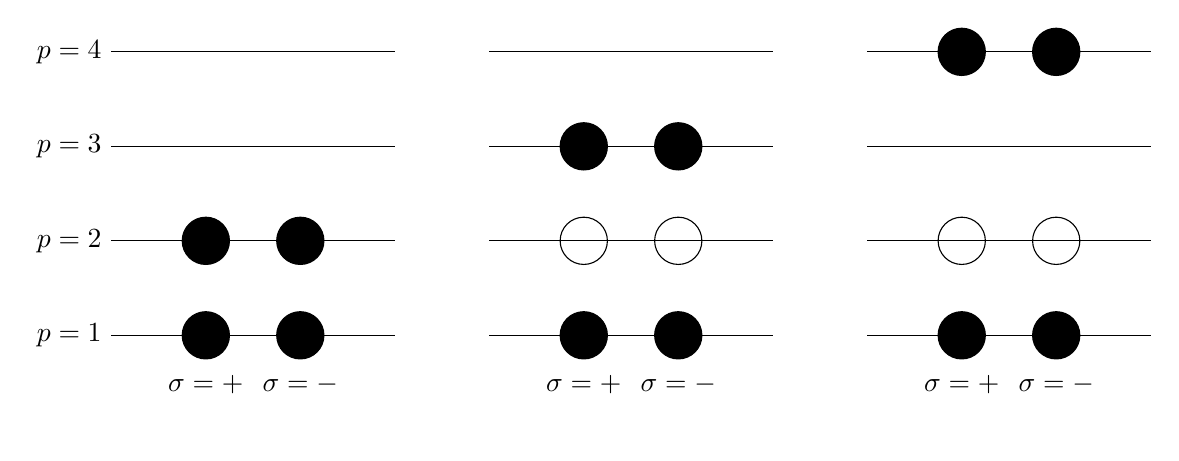
\begin{tikzpicture}[scale=1.2]
    \begin{scope}
      \foreach \i in {1,...,4}
      {
        \draw (-1,\i-1) node[anchor=east] {$p = \i$} --(2,\i-1);
      }
      \filldraw (0,0) node[anchor=north,inner sep=.5cm] {$\sigma=+$} circle (0.25cm); 
      \filldraw (1,0) node[anchor=north,inner sep=.5cm] {$\sigma=-$} circle (0.25cm);
      \filldraw (0,1) circle (0.25cm); 
      \filldraw (1,1) circle (0.25cm);
    \end{scope}
    \begin{scope}[xshift=4cm]
      \foreach \i in {1,...,4}
      {
        \draw (-1,\i-1) --(2,\i-1);
      }
      \filldraw (0,0) node[anchor=north,inner sep=.5cm] {$\sigma=+$} circle (0.25cm); 
      \filldraw (1,0) node[anchor=north,inner sep=.5cm] {$\sigma=-$} circle (0.25cm);
      \draw (0,1) circle (0.25cm); 
      \draw (1,1) circle (0.25cm);
      \filldraw (0,2) circle (0.25cm); 
      \filldraw (1,2) circle (0.25cm);
    \end{scope}
    \begin{scope}[xshift=8cm]
      \foreach \i in {1,...,4}
      {
        \draw (-1,\i-1) --(2,\i-1);
      }
      \filldraw (0,0) node[anchor=north,inner sep=.5cm] {$\sigma=+$} circle (0.25cm); 
      \filldraw (1,0) node[anchor=north,inner sep=.5cm] {$\sigma=-$} circle (0.25cm);
      \draw (0,1) circle (0.25cm); 
      \draw (1,1) circle (0.25cm);
      \filldraw (0,3) circle (0.25cm); 
      \filldraw (1,3) circle (0.25cm);
    \end{scope}
  \end{tikzpicture}
  \newline
  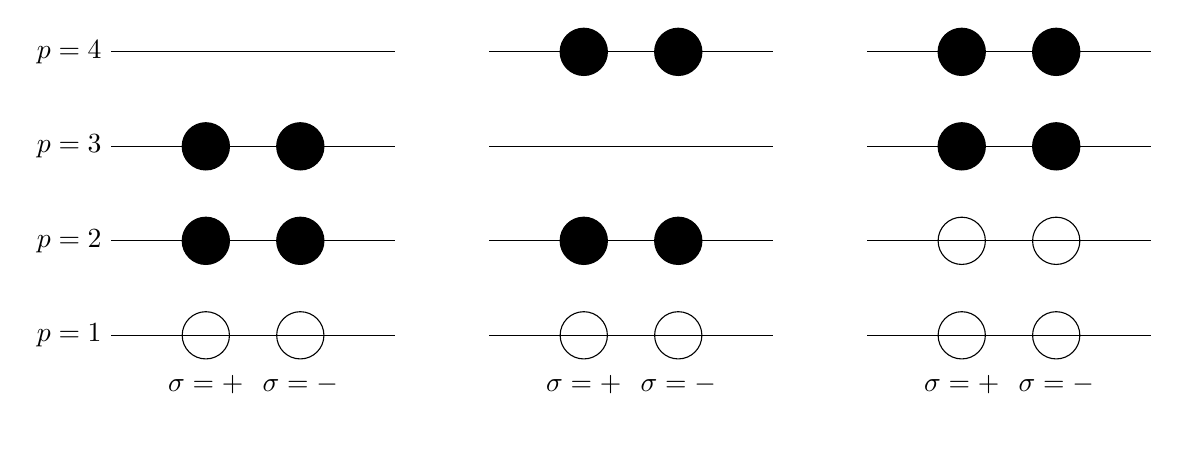
\begin{tikzpicture}[scale=1.2]
    \begin{scope}
      \foreach \i in {1,...,4}
      {
        \draw (-1,\i-1) node[anchor=east] {$p = \i$} --(2,\i-1);
      }
      \draw (0,0) node[anchor=north,inner sep=.5cm] {$\sigma=+$} circle (0.25cm); 
      \draw (1,0) node[anchor=north,inner sep=.5cm] {$\sigma=-$} circle (0.25cm);
      \filldraw (0,1) circle (0.25cm); 
      \filldraw (1,1) circle (0.25cm);
      \filldraw (0,2) circle (0.25cm); 
      \filldraw (1,2) circle (0.25cm);
    \end{scope}
    \begin{scope}[xshift=4cm]
      \foreach \i in {1,...,4}
      {
        \draw (-1,\i-1) --(2,\i-1);
      }
      \draw (0,0) node[anchor=north,inner sep=.5cm] {$\sigma=+$} circle (0.25cm); 
      \draw (1,0) node[anchor=north,inner sep=.5cm] {$\sigma=-$} circle (0.25cm);
      \filldraw (0,1) circle (0.25cm); 
      \filldraw (1,1) circle (0.25cm);
      \filldraw (0,3) circle (0.25cm); 
      \filldraw (1,3) circle (0.25cm);
    \end{scope}
    \begin{scope}[xshift=8cm]
      \foreach \i in {1,...,4}
      {
        \draw (-1,\i-1) --(2,\i-1);
      }
      \draw (0,0) node[anchor=north,inner sep=.5cm] {$\sigma=+$} circle (0.25cm); 
      \draw (1,0) node[anchor=north,inner sep=.5cm] {$\sigma=-$} circle (0.25cm);
      \draw (0,1) circle (0.25cm); 
      \draw (1,1) circle (0.25cm);
      \filldraw (0,2) circle (0.25cm); 
      \filldraw (1,2) circle (0.25cm);
      \filldraw (0,3) circle (0.25cm); 
      \filldraw (1,3) circle (0.25cm);
    \end{scope}
  \end{tikzpicture}
\end{center}
\caption{Need good caption here.\label{fig:schematic}}
\end{figure*}
From figure (\ref{fig:schematic}) one can observe that the dimension of the subspace for $M=4$ is $3+2+1=6$, which is the number of possible states. We can easily imagine that for $M=2$ we would get 1 state, with $M=5$ we would get $4+3+2+1=10$ states and so on. Thus the dimension of the subspace for an arbitrary $M$ is given by the arithmetic series
\begin{equation}
n_M=\sum_{m=1}^{M-1}(M-m).
\end{equation}

\subsection{g}


\subsection{h}
\begin{equation}
\hat{H}=\hat{H_0}+\hat{V}
\end{equation}
We use equation ... and ..., and get
\begin{align}
\hat{V}&=-\frac{1}{2}g\sum_{pq}c_{p+}^{\dagger}c_{p-}^{\dagger}c_{q-}c_{q+}\notag\\
&=-\frac{1}{2}g\sum_{p}^Mc_{p+}^{\dagger}c_{p-}^{\dagger}\sum_q^Mc_{q-}c_{q+}\notag\\
&=-\frac{1}{2}g\bigg(\sum_{p=1}^4\hat{P}_p^{\dagger}\bigg)\bigg(\sum_{q=1}^4\hat{P}_q\bigg)
\end{align}
Similarly we get
\begin{align}
\hat{H_0}&=\sum_{p\sigma}\varepsilon_pc_{p\sigma}^{\dagger}c_{p\sigma}\notag\\
&=\sum_p(p-1)\sum_{\sigma}c_{p\sigma}^{\dagger}c_{p\sigma}\notag\\
&=\sum_p(p-1)\hat{n}_p.
\end{align}
Thus we end up with
\begin{equation}
\hat{H}=\sum_p(p-1)\hat{n}_p-\frac{1}{2}g\bigg(\sum_{p=1}^4\hat{P}_p^{\dagger}\bigg)\bigg(\sum_{q=1}^4\hat{P}_q\bigg)
\end{equation}

\section{Garbage} 
\begin{table} [H]
\centering
\caption{This table represents the error when solving the system for a constant solution. }
\begin{tabularx}{\textwidth}{XXXX} \hline
\label{tab:constant_error}
Elements & 1D & 2D & 3D \\ \hline
P1 & 2.77555756e-15 & 3.55271367e-15 & 2.60902410e-14 \\
P2 & 1.26343380e-13 & 1.39666056e-13 & 8.69304628e-14 \\ \hline
\end{tabularx}
\end{table}

%\begin{figure}[H]
%\centering
%\includegraphics[width=100mm]{constant_solution_2.png}
%\caption{This figure shows the numerical solution of the constant function in 2 dimensions \label{fig:constant_error_2}}
%\end{figure}
 

\end{document}
